\documentclass[11pt,a4paper]{article}
\usepackage[czech]{babel}
\usepackage[utf8]{inputenc}
\usepackage{times}
\usepackage{url}
\usepackage[textwidth=15.2cm,textheight=23cm]{geometry}
\usepackage{xcolor}

\usepackage{graphicx}

%\usepackage{fancyvrb}
%\DefineVerbatimEnvironment{verbatim}{Verbatim}{}

\usepackage[bf]{caption}

\usepackage[hyperindex,
  plainpages=false,
  pdftex,
  colorlinks,
  pdfborder={0 0 0},
  pdfpagelabels]{hyperref}

\pdfcompresslevel=9

\newcommand{\myincludegraphics}[4]{
  \begin{figure}[!h]
  \centering
  \includegraphics[#1]{#2}
  \caption{#3.} \label{#4}
  \end{figure}
}

% titulní stránka a obsah
\newcommand{\titlepageandcontents}{
  % credits for template go to: Martin Striz
\begin{titlepage}

\vspace*{1cm}

\begin{figure}
  \centering
  
\includegraphics[height=6cm]{images/fit.pdf}
\end{figure}

\vspace*{5mm}

\begin{center}
\begin{Large}
Projekt do předmětu GMU -- Grafické a multimediální procesory
\end{Large}
\end{center}

\vspace*{5mm}

\begin{center}
\begin{Huge}
Výpočet siluet pomocí GPU \\
\end{Huge}
\end{center}

\vspace*{1cm}

\begin{center}
\begin{Large}
\today
\end{Large}
\end{center}

\vfill

\begin{flushleft}
\begin{large}
\begin{tabular}{ll}

\bf Řešitelé:\hspace{3mm} & Zdeněk Biberle (\verb_xbiber00@stud.fit.vutbr.cz_) \\
& Vít Hodes (\verb_xhodes00@stud.fit.vutbr.cz_) \\
& Fakulta Informačních Technologií \\
& Vysoké Učení Technické v~Brně

\end{tabular}
\end{large}
\end{flushleft}

\end{titlepage}

% vim:set ft=tex expandtab enc=utf8:


  \pagestyle{plain}
  \pagenumbering{roman}
  \setcounter{page}{1}
  %\tableofcontents

  \newpage
  \pagestyle{plain}
  \pagenumbering{arabic}
  \setcounter{page}{1}
}

\def\uv#1{\iflanguage{english}{``#1''}%
                              {\quotedblbase #1\textquotedblleft}}%

% vim:set ft=tex expandtab enc=utf8:


\begin{document}
\titlepageandcontents

%---------------------------------------------------------------------------
\section{Zadání}

\begin{itemize}
	\item Výpočet stínových těles
		\begin{itemize}
			\item Implementace na GPU
			\item Implementace na CPU pro porovnání rychlosti
		\end{itemize}
	\item Vytvoření demonstrační aplikace
		\begin{itemize}
			\item Vykreslení scény se stíny pomocí patřičně modifikovaného z-fail algoritmu
			\item Měření rychlosti
			\item Různé vizualizační pomůcky
		\end{itemize}
	\item Volba či vytvoření vhodných modelů pro demonstraci finálního výsledku
\end{itemize}

%---------------------------------------------------------------------------
\section{Použité technologie}

\section{Technologie potřebné pro běh}
\begin{itemize}
	\item Grafický akcelerátor s podporou OpenGL 4.3
		\begin{itemize}
			\item SSBO
			\item Image load/store
			\item Compute shadery
		\end{itemize}
	\item Knihovna SDL2
	\item Knihovna GLM
	\item Knihovna GLEW
\end{itemize}

\section{Technologie použité pro tvorbu}
\begin{itemize}
	\item Blender
	\item Textový editor/vývojové prostředí vlastní volby
\end{itemize}

%---------------------------------------------------------------------------
\section{Použité zdroje}
\begin{itemize}
	\item Stanford bunny
	\item Utah teapot
	\item Byungmoon Kim, Kihwan Kim, Greg Turk - Real Time Shadow of Transparent Casters Using Shadow Volume, 2007
	\item Dokumentace OpenGL 4.3
\end{itemize}
%---------------------------------------------------------------------------
\section{Nejdůležitější dosažené výsledky}

\subsection{Obecná funkčnost a funkcionalita aplikace}
\begin{figure}[h]
	\captionsetup{type=figure}
	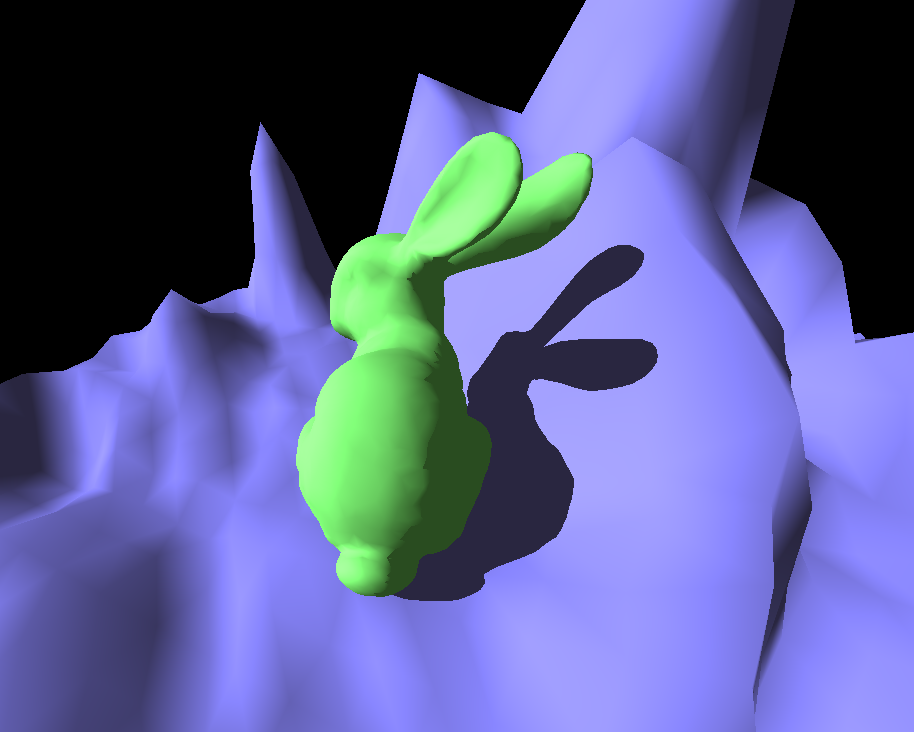
\includegraphics[width=\textwidth]{images/bunny.png}
	\captionof{figure}{Králíček vrhající stín na terén}
\end{figure}

\begin{figure}[h]
	\captionsetup{type=figure}
	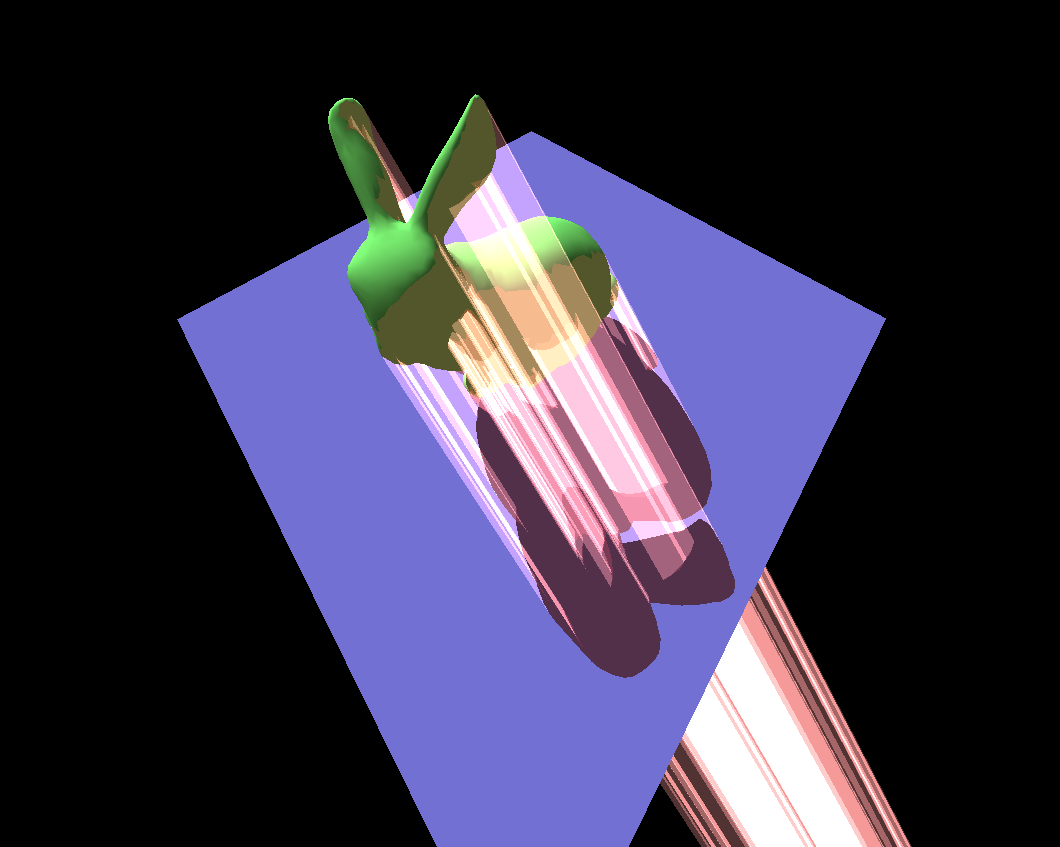
\includegraphics[width=\textwidth]{images/bunny-volume.png}
	\captionof{figure}{Králíček a jeho stínové těleso}
\end{figure}

Aplikace provádí generování stínového tělesa pro libovolný model na CPU i na GPU a scénu poté zobrazuje s jeho použitím. Dodatečně umožňuje i zobrazení samotného stínového tělesa. Ovšem dle našich zkušeností nefunguje generování stínového tělesa na grafických kartách od společnosti AMD.

\subsection{Generování stínových těles i pro non-manifold geometrii}

\begin{figure}[h]
	\captionsetup{type=figure}
	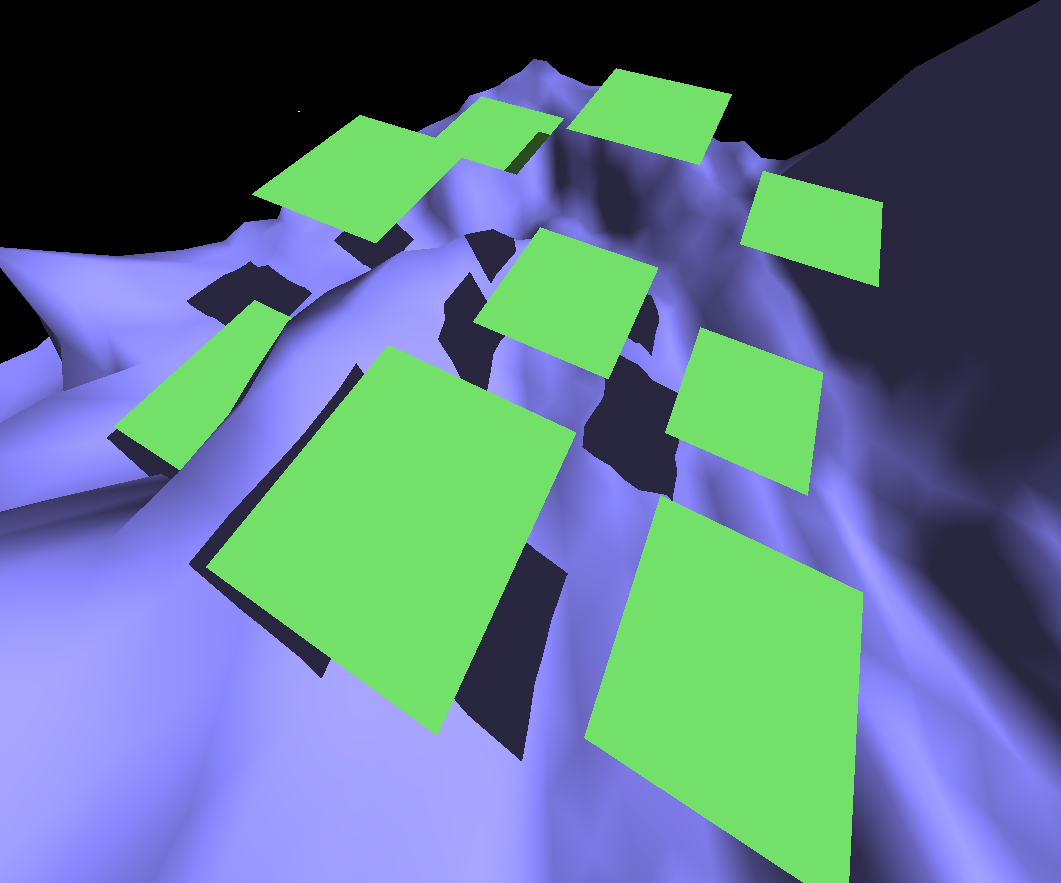
\includegraphics[width=\textwidth]{images/multiple-raised-planes.png}
	\captionof{figure}{Geometrie složená z několika non-manifold částí vrhající stíny}
	\label{fig:multiple-raised-planes}
\end{figure}

Zadaný algoritmus umožňuje generování stínových těles i pro non-manifold geometrii. Na obrázku \ref{fig:multiple-raised-planes} vidíme několik čtverců vrhajících korektní stín. Každý tento čtverec je složen pouze ze dvou trojúhelníků a není tedy možné na ně aplikovat běžný algoritmus generování stínových těles (tj. protažení hran mezi dvěma trojúhelníky, kde jeden je natočen ke světlu a druhý je od světla odvrácen) tak, aby dosáhl správného výsledku.

\subsection{Zrychlení GPU implementace}

Měřením času provádění CPU i GPU implementace při použití různých modelů jsme získali následující data:

\begin{tabular}{l|c|c|c|c}
	Název modelu   & Počet trojúhelníků  & CPU - čas  & GPU - čas & Zrychlení GPU oproti CPU \\
	\hline
	cube.obj       & 12      & 0,931 ms   & 0,195 ms  & 0,210 \\
	terrain.obj    & 1458    & 4,973 ms   & 1,302 ms  & 3,820 \\ 
	bunny.obj      & 4968    & 15,015 ms  & 2,095 ms  & 7,167 \\
	teapot.obj     & 36096   & 0,107 s    & 7,135 ms  & 15,023 \\
	teapot-big.obj & 324864  & 0,949 s    & 50,974 ms & 18,620 \\
\end{tabular}

Měření bylo provedeno na jediném počítači s grafickou kartou od společnosti nVidia, který jsme měli k dispozici. Jeho HW a SW vybavení bylo následující:
\begin{itemize}
	\item CPU: Intel Core i5-3230M, 2,60 GHz
	\item GPU: nVidia 730M
	\item RAM: 4 GiB DDR3 1.6 GHz
	\item Operační systém: Arch Linux, jádro linux-ck 3.18.1-8
	\item Ovladač GPU: nvidia-ck, 343.36-3
\end{itemize}

Ze získaných výsledků vidíme očekávanou neefektivitu GPU implementace pro modely s opravdu nízkým počtem trojúhelníků, která je pravděpodobně způsobena dodatečnou režií. V případě většího počtu trojúhelníků již ovšem vidíme znatelné urychlení činnosti, zjevně stoupající s počtem trojúhelníků.

\section{Obecný popis implementace algoritmu tvorby stínového tělesa}

Algoritmus pro každý trojúhelník stínícího objektu provede následující:
\begin{itemize}
	\item Zkontroluje, zda je trojúhelník natočen ke světlu. Pokud ano, tak jej přenese do výstupního bufferu a zároveň přidá i patřičně upravenou verzi tohoto trojúhelníku na konci stínového tělesa.
	\item Pro každou hranu tohoto trojúhelníku provede následující:
		\begin{itemize}
			\item Binárním vyhledáváním nalezne v pomocném poli pro vyhledávání trojúhelníků všechny ostatní trojúhelníky, které sdílí tuto hranu.
			\item Zkontroluje, zda je tento trojúhelník vlastníkem této hrany (tj. neexistuje trojúhelník, který sdílí tuto hranu a má nižší index). Pokud tomu tak není, tak přejde na další hranu.
			\item Projde nalezené přilehlé trojúhelníky a na základě jejich pozice v prostoru vůči světlu spočítá multiplicitu hrany. 
			\item Pokud výsledná multiplicita není nulová, tak hranu protáhne a přenese do výstupního bufferu.
		\end{itemize}
\end{itemize}

%---------------------------------------------------------------------------
\section{Ovládání vytvořeného programu}

\begin{itemize}
	\item Levé tlačítko myši - Společně s pohybem myši umožňuje změnu úhlu pohledu na scénu.
	\item Kolečko myši - Přiblížení a oddálení zobrazené scény.
	\item Klávesa R - Přepíná autonomní otáčení zobrazené scény.
	\item Klávesa T - Přepíná zobrazení vypočteného stínového tělesa.
	\item Klávesa C - Přepíná mezi CPU a GPU implementací výpočtu stínového tělesa.
\end{itemize}

%---------------------------------------------------------------------------
\section{Zvláštní použité znalosti}

Použití OpenGL compute shaderů se různě liší od použití OpenCL či CUDA. To vyžadovalo získání dodatečných informací o jejich využívání a o komunikaci s nimi. Dále také využití image load/store v OpenGL shaderech pro vytvoření vlastního "stencil bufferu".

%---------------------------------------------------------------------------
\section{Rozdělení práce v týmu}

\paragraph{Zdeněk Biberle} Základ aplikace, GPU výpočet stínového tělesa, CPU výpočet stínového tělesa, dokumentace.
\paragraph{Vít Hodes} Vykreslení scény za použití stínového tělesa, nahrávání modelů, CPU výpočet stínového tělesa.

%---------------------------------------------------------------------------
\section{Co bylo nejpracnější}

\paragraph{Zdeněk Biberle}
Značnou část času jsem strávil nad komunikací mezi aplikací a compute shaderů. Později jsem zjistil, že implementace SSBO na grafických kartách od AMD se v současnosti vyznačuje různými problémy a tudíž jsem řešil nevyřešitelné. Náročné bylo také vymyslet, jak vygenerovaná data použít pro z-fail algoritmus. To se nám ovšem ve finále úspěšně nepodařilo a ve výsledné aplikaci je tak použit algoritmus z-pass.

\paragraph{Vít Hodes} Přijít na to, jak implementovat celočíselný "stencil buffer" s obecným přístupem ze shaderů. Po prozkoumání několika slepých cest se dospělo k řešení pomocí iimage2D a atomického sčítání. Taktéž implementovat stíny nad shadow volume, který se mi na AMD kartě negeneruje správně se moc nedá.

%---------------------------------------------------------------------------
\section{Zkušenosti získané řešením projektu}

\paragraph{Zdeněk Biberle}
\begin{itemize}
	\item Compute shadery
	\item SSBO
	\item Image load/store
\end{itemize}

\paragraph{Vít Hodes}
\begin{itemize}
	\item Framebuffer object, color/depth attachment
	\item V GLSL existují i shadow samplery a image samplery
	\item Image load/store, atomické operace obecně v shaderech
	
\end{itemize}

%---------------------------------------------------------------------------
\section{Autoevaluace}

\paragraph{Technický návrh (75\%):}
Technický návrh je slušný, problém byl vhodně rozložen na podproblémy, snad jen samotný výpočet stínového tělesa mohl být dodatečně rozdělen na dvě části (jedna zpracovávající trojúhelníky a druhá zpracovávající hrany).


\paragraph{Programování (65\%):} 
Vzhledem ke kratšímu rozsahu se moc neuplatňuje zapouzdření ve vykreslovací části. Znovupoužitelnost
spíše znalostí než konkrétního kódu. Mimo vykreslovací část je kód poměrně dobře čitelný.

\paragraph{Vzhled vytvořeného řešení (40\%):} 
Estetická kvalita nebyla cílem řešení.

\paragraph{Využití zdrojů (80\%):} Byl využit pouze jeden literární zdroj, což je ovšem pro tento projekt dostatečné. Veškerý kód je původní a při jeho tvorbě byla značně využívána dokumentace OpenGL.

\paragraph{Hospodaření s časem (70\%):} (rovnoměrné dotažení částí projektu,
míra spěchu, chybějící části řešení, $\ldots$)
Od počátku prací na projektu byl postup přiměřený a stabilní. Mohlo ovšem být věnováno více času implementaci algoritmu z-fail.

\paragraph{Spolupráce v týmu (80\%):}
Komunikace a spolupráce byla z obou stran dobrá.

\paragraph{Celkový dojem (70\%):}
Projekt byl zajímavý a potenciálně velmi užitečný. Škoda problémů s různými platformami (AMD x nVidia).

%---------------------------------------------------------------------------
\section{Doporučení pro budoucí zadávání projektů}

Témata projektů byla dostatečně pestrá, ale příště by mohla být zadána dříve. Ovšem na druhou stranu se řešení tohoto projektu příliš nepřekrývalo s jinými projekty v semestru.

%---------------------------------------------------------------------------

\end{document}
% vim:set ft=tex expandtab enc=utf8:
